\documentclass[12pt]{article}
\usepackage{amsmath}
\usepackage{amssymb}
\usepackage{amsthm}
\usepackage{cancel}
\usepackage{enumitem}
\usepackage{esdiff}
\usepackage{graphicx}
\usepackage[version=4,textfontname=sffamily,mathfontname=mathsf]{mhchem}
\usepackage{multicol}
\usepackage{siunitx}
\usepackage{ulem}
% \usepackage{pgfplots}
\usepackage{wrapfig}
\usepackage{xcolor}

\newcommand{\e}[1]{e^{#1}}
\newcommand{\ei}[1]{e^{i\left(#1\right)}}
\newcommand{\E}[1]{\times 10^{#1}}
\newcommand{\tagref}[1]{\tag{\ref{#1}}}

\renewcommand\qedsymbol{TENA}

\title{
    Homework \#14
    \\  \small
    PHYS 4D: Modern Physics
    \\
    Problems from Krane's textbook
    }
\author{Donald Aingworth IV}
\date{April 27, 2026}

\begin{document}
\maketitle
\DeclareSIUnit{\amu}{amu}
\DeclareSIUnit{\light}{c}
\DeclareSIUnit{\lightyear}{c\cdot yr}
\DeclareSIUnit{\year}{yr}
\DeclareSIUnit{\yr}{yr}

\section{Questions, Chapter 2}
    \subsection{Question 15}
        Suppose event A causes event B. 
        To one observer, event A comes before event B. 
        Is it possible that in another frame of reference event B could come before event A? 
        Discuss.

        \subsubsection{Answer}
            \begin{wrapfigure}{r}{0.25\textwidth}
                \vspace{-30pt}
                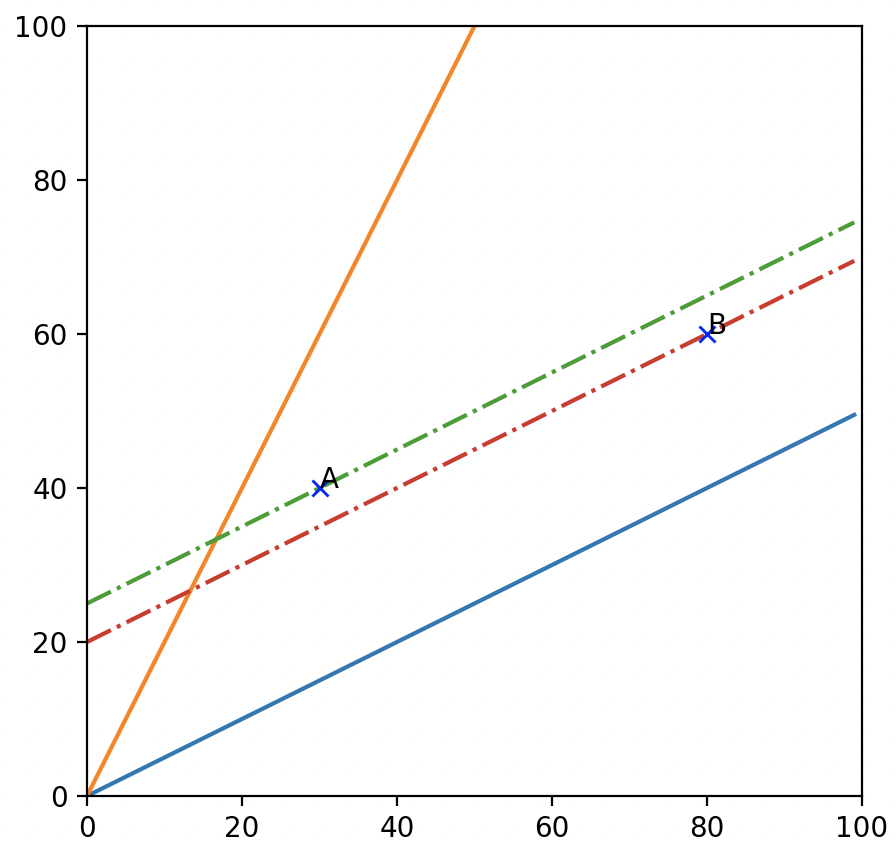
\includegraphics[width=0.25\textwidth]{Answers Images/Q15a.png} 
                \label{fig:11.11}
            \end{wrapfigure}
            I initially thought that this is possible.
            Suppose event B takes place significantly farther away but only slightly after event A.
            This is pictured to the right. 
            Point B occurs after event A, taking the vertical axis as time, but it takes place significantly farther away.
            Looking at the point in time at which the moving observer would see each event occur, they would see event B happen before event A.
            That seems to imply that it is possible, right?

            The issue comes when you remember that event B is caused by event A.
            For this to be the case here, whatever made event A cause event B (e.g. a photon from event A hitting the things the member parts of event B) would have to be traveling faster than light.
            This would then imply that it is impossible.
            Conclusively, as long as no object or information can travel faster than the speed of light, the answer is no, event A will not appear to happen after event B.
        \pagebreak

    \subsection{Question 17}
        ``In special relativity, mass and energy are equivalent.''
        Discuss this statement and give examples.

        \subsubsection{Answer}
            This refers to how mass and energy are very closely related within the context of special relativity.
            One example is that the rest energy of an object is directly proportional to the mass ($E_0 = mc^2$).
            It also refers to how objects (specifically quantum objects) colliding at very high speeds may form different objects whose total mass is different from the total mass of the initial objects that formed it but whose total energy (rest energy included) will be the same.

    \subsection{Question 19}
        Could a collision be elastic in one frame of reference and inelastic in another?

        \subsubsection{Answer}
            No.
            Let's set up the equations for an elastic collision.
            First momentum.
            \begin{gather}
                p_{1i} + p_{2i} = p_{1f} + p_{2f}\\
                \frac{m_1 v_{1i}}{\sqrt{1 - v_{1i}^2/c^2}} + \frac{m_2 v_{2i}}{\sqrt{1 - v_{2i}^2/c^2}} = \frac{m_1 v_{1f}}{\sqrt{1 - v_{1f}^2/c^2}} + \frac{m_2 v_{2f}}{\sqrt{1 - v_{2f}^2/c^2}}
            \end{gather}

            Then kinetic energy.
            \begin{gather}
                K_{1i} + K_{2i} = K_{1f} + K_{2f}\\
                \frac{m_1 c^2}{\sqrt{1 - v_{1i}^2/c^2}} + \frac{m_2 c^2}{\sqrt{1 - v_{2i}^2/c^2}} = \frac{m_1 c^2}{\sqrt{1 - v_{1f}^2/c^2}} + \frac{m_2 c^2}{\sqrt{1 - v_{2f}^2/c^2}}
            \end{gather}

            For a different frame of reference, we can suppose we change the velocity value according to the Lorentz transformation.
            In either case, we have a consistent equation for the energy.
            The total energy in a collision will be the same.
            Assuming the total mass to be the same, the total rest energy will be constant.
            Since total rest energy remains constant, that also means that total kinetic energy will remain constant.
            As such, the collision will remain elastic.
    \pagebreak

\section{Problem 17} % 2.5
    A neutral K meson at rest decays into two $\pi$ mesons, which travel in opposite directions along the x axis with speeds of $0.828c$. 
    If instead the K meson were moving in the positive x direction with a velocity of $0.486c$, what would be the velocities of the two $\pi$ mesons?

    \subsection{Solution}
        This uses a Lorentz transformation along th $x$-axis.
        \begin{equation}
            v_x' = \frac{v_x - u}{1 - v_xu/c^2}
        \end{equation}

        Within the frame moving at the same speed as the K meson, the two $\pi$ mesons appear to traveling in opposite directions at a speed of $0.828c$.
        Suppose we consider the speed of the new frame $u = -0.486c$.
        We can calculate the value of $v_x'$, first for the one traveling in the $+x$ direction.
        \begin{equation}
            v_x'    =   \frac{v_x - u}{1 - v_xu/c^2}
                =   \frac{0.828c + 0.486c}{1 + 0.828*0.486}
                =   \frac{1.314}{1.402408} c
                =   \boxed{0.937c}
        \end{equation}

        Now the velocity of the meson in the opposite direction.
        \begin{equation}
            v_x'    =   \frac{v_x - u}{1 - v_xu/c^2}
                =   \frac{-0.828c + 0.486c}{1 - 0.828*0.486}
                =   -\frac{0.342}{0.597592} c
                =   \boxed{-0.5723c}
        \end{equation}
    \pagebreak

\section{Problem 18}
    A rod in the reference frame of observer $O$ makes an angle of $31\unit{\degree}$ with the $x$ axis. 
    According to observer $O'$, who is in motion in the $x$ direction with velocity $u$, the rod makes an angle of $46\unit{\degree}$ with the $x$ axis. 
    Find the velocity $u$.

    \subsection{Solution}
        If $O'$ is only moving along the $x$ axis, we don't even need to use the Lorentz transformation.
        Suppose the rod has a length $\ell$.
        In the $x$-axis from $O$, the rod extends a distance of $\ell\cos(31\unit\degree)$, which can be our value of $L_o$.
        In the $x$-axis from $O'$, the rod extends a distance of $\ell\cos(46\unit\degree)$, which can be our value of $L$.
        From here, we can use the length transformation equation to find $u$.
        \begin{gather}
            L = L_o \sqrt{1 - u^2/c^2}\\
            \frac{L^2}{L_o^2} = 1 - u^2/c^2\\
            \frac{u^2}{c^2} =   1 - \frac{L^2}{L_o^2}
                =   1 - \frac{\cos^2(46\unit\degree)}{\cos^2(31\unit\degree)}
                =   1 - \frac{0.48255}{0.73474}
                =   0.34323\\
            \boxed{u = 0.58586c}
        \end{gather}
    \pagebreak

\section{Problem 24} % 2.6
    \begin{wrapfigure}{r}{0.25\textwidth}
        \vspace{-30pt}
        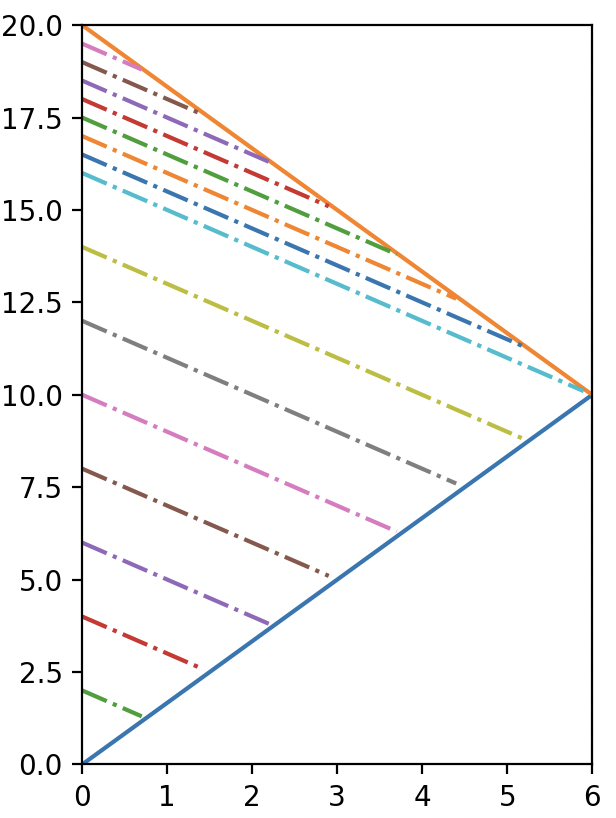
\includegraphics[width=0.25\textwidth]{Answers Images/P24a.png} 
        \label{fig:2.24.a}
    \end{wrapfigure}
    Make a drawing similar to Figure 2.20 showing the worldlines of Casper and Amelia from Casper's frame of reference.
    Divide the world line for Amelia's outward journey into 8 equal segments (for the 8 birthdays that Amelia celebrates).
    For each birthday, draw a line that represents a light signal that Amelia sends to Casper on her birthday. 
    Do the same for Amelia's return journey. 
    (a) According to Casper's time, when does he receive the signal showing Amelia celebrating her 8th birthday after leaving Earth? 
    (b) How long does it take for Casper to receive the signals showing Amelia celebrating birthdays 9 through 16?

    \subsection{Solution (a)}
        My graph requested is above and to the right, made using MatPlotLib since I don't like drawing and I don't care about colors.
        Each colorful dashed line is one birthday.
        Casper receives Amelia's 8th birthday celebration around year 16. 

    \subsection{Solution (b)}
        After Amelia's 8th birthday, each birthday celebration would be received at intervals of around half a year, over the course of four years.

    \pagebreak

\section{Problem 26} % 2.7
    Find the (a) momentum, (b) kinetic energy, and (c) total energy of a proton moving at a speed of $0.756c$.

    \subsection{Solution (a)}
        Momentum has a simple formula.
        \begin{equation}
            \vec{p} = \frac{m\vec{v}}{\sqrt{1 - v^2/c^2}}
        \end{equation}

        The mass of the proton is $938.272\,\unit{\mega\eV/\light^2}$.
        We can use this to find the momentum.
        \begin{equation}
            p   =   \frac{938.272\,\unit{\mega\eV/\light} * 0.756}{\sqrt{1 - 0.756^2}}
                =   \frac{709.333632\,\unit{\mega\eV/\light}}{0.6546}
                =   \boxed{1083.66\,\unit{\mega\eV/c}}
        \end{equation}

    \subsection{Solution (b)}
        Kinetic energy also has a formula.
        \begin{align}
            K   &=  \frac{mc^2}{\sqrt{1 - v^2/c^2}} - mc^2
                =   \frac{938.272\,\unit{\mega\eV}}{\sqrt{1 - 0.756^2}} - 938.272\,\unit{\mega\eV}\\
                &=  \frac{938.272\,\unit{\mega\eV}}{0.6546} - 938.272\,\unit{\mega\eV}
                =   1433.414\,\unit{\mega\eV} - 938.272\,\unit{\mega\eV}\\
                &=  \boxed{495.14\,\unit{\mega\eV}}
        \end{align}

    \subsection{Solution (c)}
        Total energy has a formula.
        \begin{gather}
            E^2 = (pc)^2 + (mc^2)^2\\
            \begin{align}
                E   &=  \sqrt{(pc)^2 + (mc^2)^2}
                    =   \sqrt{(1083.66\,\unit{\mega\eV})^2 + (938.272\,\unit{\mega\eV})^2}\\
                    &=  \sqrt{1 174 318.9956 + 880 354.345984}\,\unit{\mega\eV}
                    =   \sqrt{2 053 243.345984}\,\unit{\mega\eV}\\
                    &=  \boxed{1.432914\,\unit{\giga\eV}}
            \end{align}
        \end{gather}
    \pagebreak

\section{Problem 37}
    An electron and a proton are each accelerated starting from rest through a potential difference of 10.0 million volts. 
    (a) Find the momentum (in MeV/c) and the kinetic energy (in MeV) of each, and (b) compare with the results of using the classical formulas.

    \subsection{Solution}
        The kinetic energy of an electron after going through 10 million volts would be 10 MeV, and the same for the proton.
        This is the case both classically and relativistically.
        Relativistically, we have a handful of formulas for the momentum and related to the kinetic energy.
        \begin{gather}
            E \approxeq pc\\
            E = K + mc^2; E^2 = (pc)^2 + (mc^2)^2\\
            (pc)^2 = (K + mc^2)^2 + (mc^2)^2
        \end{gather}
        
        For the electron first.
        \footnotesize
        \begin{align}
            p   &=  \frac{1}{c} \sqrt{(K + mc^2)^2 + (mc^2)^2}
                =   \sqrt{(10\,\unit{\mega\eV} + 0.511\,\unit{\mega\eV})^2 + (0.511\,\unit{\mega\eV})^2}\,\unit{\light^{-1}}\\
                &=  \sqrt{(10.511\,\unit{\mega\eV})^2 + (0.511\,\unit{\mega\eV})^2}\,\unit{\light^{-1}}
                =   \sqrt{110.48\E{12}\,\unit{\eV} + 100\E{12}\,\unit{\eV}}\\
                &=   \sqrt{210.48\E{12}\,\unit{\eV}}\,\unit{\light^{-1}}
                =  \boxed{14.5\,\unit{\mega\eV/\light}}
        \end{align}
        \normalsize

        Now the proton.
        \footnotesize
        \begin{align}
            p   &=  \frac{1}{c} \sqrt{(K + mc^2)^2 + (mc^2)^2}
                =   \sqrt{(10\,\unit{\mega\eV} + 938.3\,\unit{\mega\eV})^2 + (938.3\,\unit{\mega\eV})^2}\,\unit{\light^{-1}}\\
                &=  \sqrt{(948.3\,\unit{\mega\eV})^2 + (938.3\,\unit{\mega\eV})^2}\,\unit{\light^{-1}}
                =   \sqrt{880.4\E{15}\,\unit{\eV} + 899.3\E{15}\,\unit{\eV}}\\
                &=   \sqrt{1.7797\E{18}\,\unit{\eV}}\,\unit{\light^{-1}}
                =  \boxed{1334\,\unit{\mega\eV/\light}}
        \end{align}
        \normalsize

    \subsection{Solution (b)}
        We have a handful of classical equations involving energy and linear momentum.
        \begin{gather}
            p = mv;
            K = \frac{1}{2}mv^2 = \frac{p^2}{2m}\\
            p = \sqrt{2mK}
        \end{gather}

        First compute the momentum of the electron.
        \begin{align}
            p   &=  \sqrt{2mK}
                =   \sqrt{2 * 0.511\,\unit{\mega\eV/\light^2} * 10\,\unit{\mega\eV}}\\
                &=  \sqrt{10.22\,\unit{\mega\eV^2/\light^2}}
                =   \boxed{3.20\,\unit{\mega\eV/c}}
        \end{align}

        Now the proton.
        \begin{align}
            p   &=  \sqrt{2mK}
                =   \sqrt{2 * 938.3\,\unit{\mega\eV/\light^2} * 10\,\unit{\mega\eV}}\\
                &=  \sqrt{18766\,\unit{\mega\eV^2/\light^2}}
                =   \boxed{137.0\,\unit{\mega\eV/c}}
        \end{align}
        
        These are \textit{very} different values from the ones calculated using relativistic formulas.
    \pagebreak

\section{Problem 40} % 2.8
    An electron and a positron (an antielectron) make a head-on collision, each moving at $v = 0.99999c$. 
    In the collision the electrons disappear and are replaced by two muons ($mc^2 = 105.7\,\unit{\mega\eV}$), which move off in opposite directions. 
    What is the kinetic energy of each of the muons?

    \subsection{Solution}
        First find the energy of the electron and positron.
        They will be identical.
        \begin{align}
            E   &=  \frac{mc^2}{\sqrt{1 - v^2/c^2}}
                =   \frac{0.511\,\unit{\mega\eV}}{\sqrt{1 - 0.99999^2}}
                =   \frac{0.511\,\unit{\mega\eV}}{\sqrt{19.9999\E{-6}}}\\
                &=  \frac{0.511\,\unit{\mega\eV}}{4.4721\E{-3}}
                =   114.26\,\unit{\mega\eV}
        \end{align}

        Since two particles identical in every relevant factor are used and two identical particles are created, we can subtract the rest energy of the two muons to find the kinetic energy of the muons.
        \begin{align}
            K   &=  E - E_0
                =   114.26\,\unit{\mega\eV} - 105.7\,\unit{\mega\eV}
                =   \boxed{8.56\,\unit{\mega\eV}}
        \end{align}
    \pagebreak

\section{Problem 41}
    It is desired to create a particle of mass 9700 \unit{\mega\eV/\light^2} in a head-on collision between a proton and an antiproton (each having a mass of 938.3 \unit{\mega\eV/\light^2}) traveling at the same speed.
    What speed is necessary for this to occur?

    \subsection{Solution}
        Let's assume it only creates one particle.
        It will be created immobile so that total momentum is is conserved.
        If the two beginning particles are traveling at the same speed and are of the same mass, each will contribute the same amount of energy.
        The net mass created by each member of the transformation will be $4850\,\unit{\mega\eV/\light^2}$, which corresponds to $4850\,\unit{\mega\eV}$.
        From there, we can find the total necessary relativistic energy and solve of the necessary velocity.
        \begin{gather}
            E = \frac{mc^2}{\sqrt{1 - v^2/c^2}}\\
            \sqrt{1 - v^2/c^2} = \frac{mc^2}{E}\\
            1 - v^2/c^2 = \frac{(mc^2)^2}{E^2}\\
            \frac{v^2}{c^2} = 1 - \frac{(mc^2)^2}{E^2}\\
            \begin{align}
                \frac{v}{c} &=  \sqrt{1 - \frac{(938.3\,\unit{\mega\eV})^2}{(4850\,\unit{\mega\eV})^2}}
                    =   \sqrt{1 - (193.46\E{-3})^2}\\
                    &=  \sqrt{1 - 0.0374}
                    =   \sqrt{0.9626}
                    =   0.9811
            \end{align}\\
            v = \boxed{0.9811c}
        \end{gather}
\end{document}